\documentclass[a4paper,12pt]{article}
\usepackage{amsmath,amssymb}
\usepackage{graphicx}
\usepackage{scaladefs}
\usepackage{scalit}
\usepackage{fancyhdr}
\pagestyle{fancy}
\lhead{\today}
\rhead{markup/blocks.nw}
\begin{document}
\section{Extracting blocks from marked up files}
While the markup intermediary format\footnote{described in the file
\texttt{markup/markup.nw}} provides a base to write all sorts of filters,
both for tangle and weave we will be required to have a more high-level
view of a literate program. The following classes will provide this
view in form of blocks.

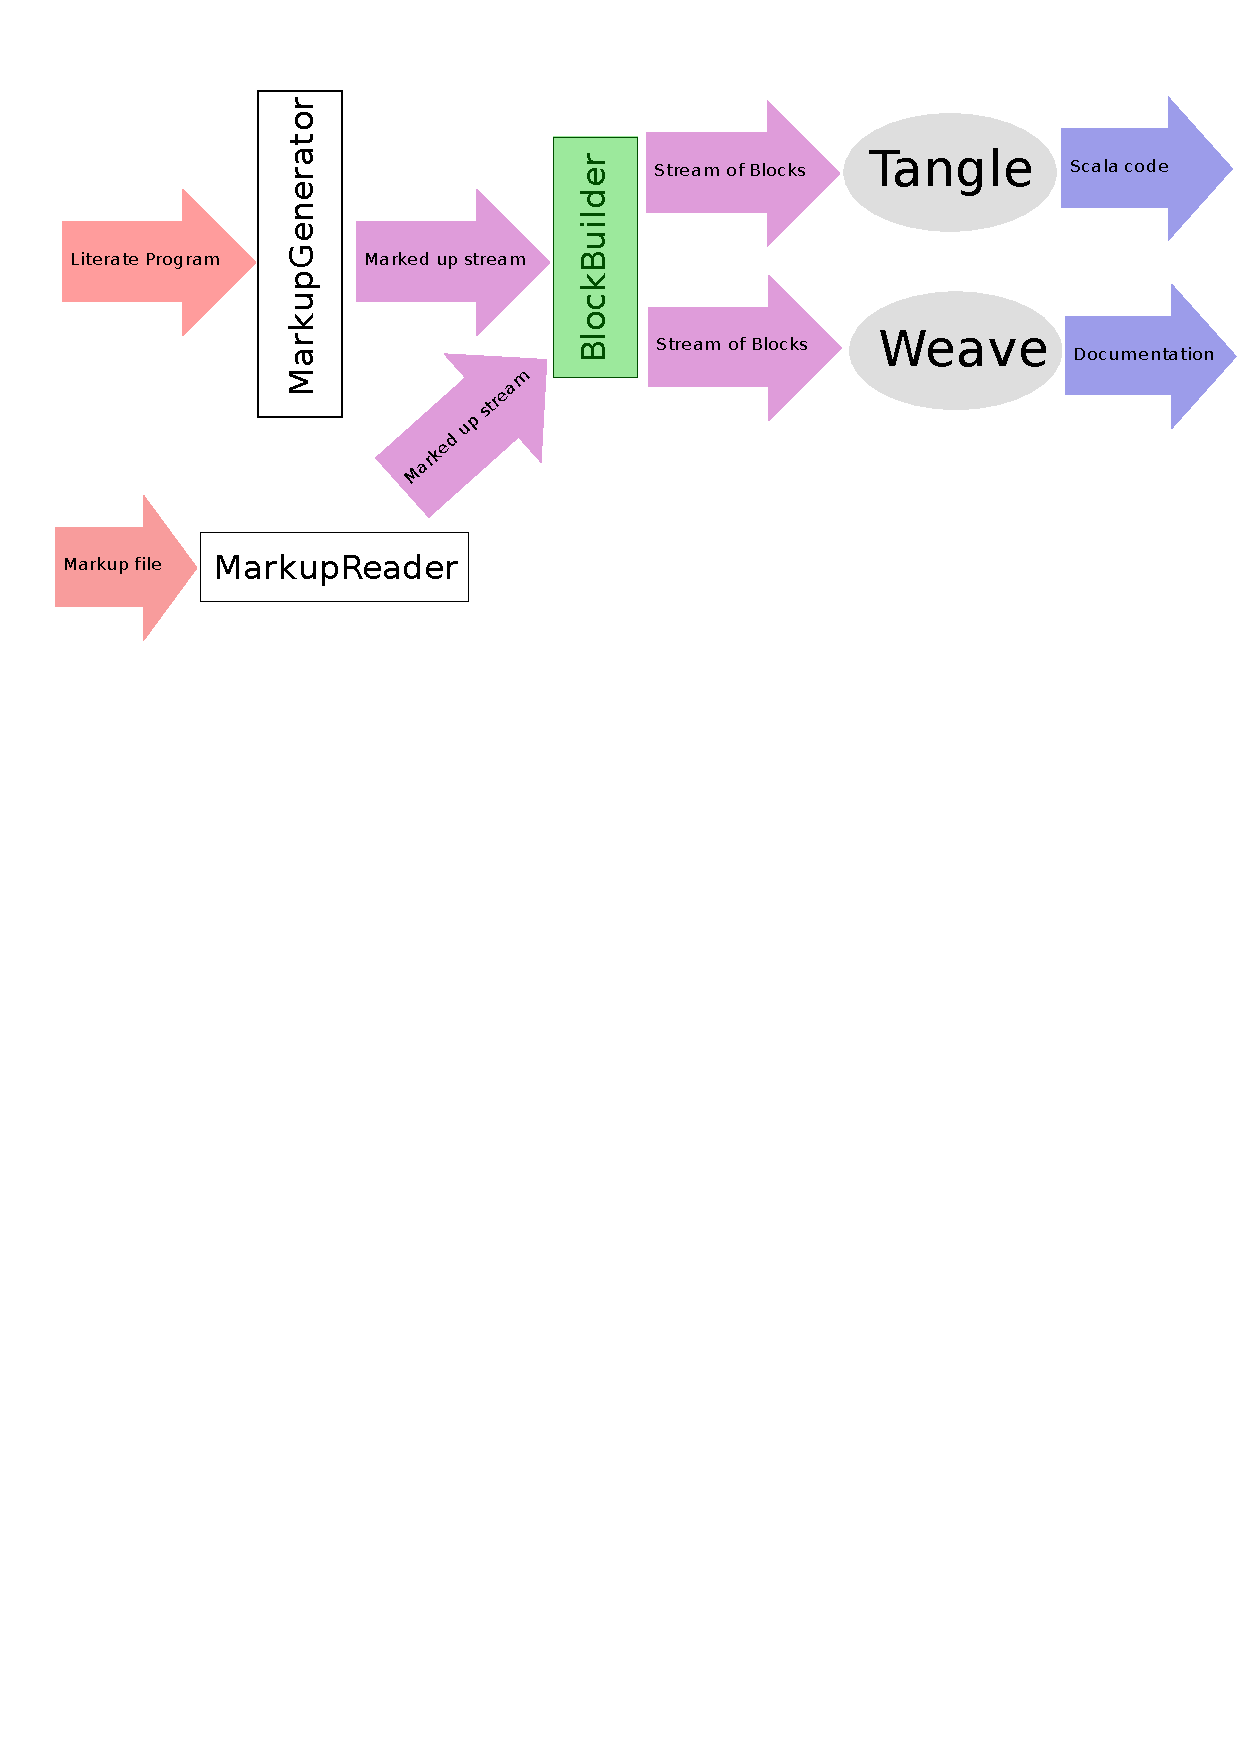
\includegraphics[width=10cm,viewport=167 590 508 800,clip]{images/blockBuilder}

$\left<\mbox{\emph{*}}\right>\equiv$
\begin{program}{\vem package}~scalit.markup
\\[0.5em]$<$Combining~strings~and~references$>$
\\[0.5em]$<$The~block~format$>$
\\[0.5em]$<$Build~blocks$>$
\\[0.5em]$<$Test~the~block~format$>$
\\[0.5em]\end{program}


\subsection{The block format}
The aim of the block format is to store the information associated with a block
(their name, chunk number, line number) while providing easy access to the
string representation their content for weave. The only thing common between
code and documentation blocks are:

\begin{itemize}
\item Block number
\item Beginning line number
\end{itemize}

$\left<\mbox{\emph{The block format}}\right>\equiv$
\begin{program}{\vem sealed}~{\vem abstract}~{\vem class}~Block$($blocknumber\,{\rm :}~Int,~linenumber\,{\rm :}~Int,
\\~~~~~~~~~~~~~~~~~~~~~~~~~~~~~~~~~~~~~~~~~~~~~~~~~~~~~~~~content\,{\rm :}~Stream$[$Line$]$$)$~{\small\{}
\\~~~~~~$<$body~of~the~block~{\vem class}$>$
\\{\small\}}
\\[0.5em]\end{program}\classdefinition{Block}
\valuedefinition{Block}{blocknumber}
\valuedefinition{Block}{linenumber}
\valuedefinition{Block}{content}



For the string representation, we run into a problem: While during tangling
we want to extract references to other code blocks, this is not the case
when we want to create documentation: Here we only want to see the name.
Another problem arises with quoted strings (that occur in documentation blocks):
Their content will be output verbatim in the documentation and deserves another
treatment. The solution here is to have a stream that can contain either
strings, references to other blocks or quoted strings.

$\left<\mbox{\emph{Combining strings and references}}\right>\equiv$
\begin{program}{\vem object}~StringRefs~{\small\{}
\\~~~~{\vem sealed}~{\vem abstract}~{\vem class}~StringRef
\\~~~~{\vem case}~{\vem class}~RealString$($content\,{\rm :}~String,
\\~~~~~~~~~~~~~~~~~~~~~~~~~~~~~~~~~~~~from\,{\rm :}~Int,
\\~~~~~~~~~~~~~~~~~~~~~~~~~~~~~~~~~~~~to\,{\rm :}~Int$)$~{\vem extends}~StringRef
\\~~~~{\vem case}~{\vem class}~QuotedString$($content\,{\rm :}~String$)$~{\vem extends}~StringRef
\\~~~~{\vem case}~{\vem class}~BlockRef$($referenced\,{\rm :}~CodeBlock$)$~{\vem extends}~StringRef
\\[0.5em]~~~~{\vem implicit}~{\vem def}~realString2string$($rs\,{\rm :}~RealString$)$~=~rs.content
\\{\small\}}
\\[0.5em]\end{program}\classdefinition{StringRef}
\classdefinition{RealString}
\classdefinition{QuotedString}
\classdefinition{BlockRef}
\objectdefinition{StringRefs}
\methoddefinition{StringRefs}{realString2string}
\valuedefinition{RealString}{content }
\valuedefinition{RealString}{from }
\valuedefinition{RealString}{to }
\valuedefinition{QuotedString}{content }
\valuedefinition{BlockRef}{referenced }



With these three different contents, we are able to define a method
that, given a map of code blocks (for dereference) will give us a
stream of \texttt{StringRef}:

$\left<\mbox{\emph{body of the block class}}\right>\equiv$
\begin{program}{\vem import}~StringRefs.\_
\\[0.5em]{\vem def}~stringRefForm$($codeBlocks\,{\rm :}~Map$[$String,CodeBlock$]$$)${\rm :}~Stream$[$StringRef$]$
\\[0.5em]\end{program}\methoddefinition{Block}{stringRefForm}



\subsubsection{Code blocks}
With this class, we can now represent the content of code blocks.
One special field is the reference to the next block: We will not
know this in the beginning, but when everything is read in, it
can be calculated.

Given a map of code blocks and their associated name, we can also
easily give back the stream of \texttt{StringRef}s:

$\left<\mbox{\emph{The block format}}\right>+\equiv$
\begin{program}{\vem case}~{\vem class}~CodeBlock$($blocknumber\,{\rm :}~Int,~linenumber\,{\rm :}~Int,
\\~~~~~~~~~~content\,{\rm :}~Stream$[$Line$]$,~blockname\,{\rm :}~String$)$
\\~~~~~~~~~~~~~~{\vem extends}~Block$($blocknumber,linenumber,content$)$~{\small\{}
\\~~~~{\vem import}~StringRefs.\_
\\~~~~{\vem override}~{\vem def}~stringRefForm$($
\\~~~~~~~~codeBlocks\,{\rm :}~Map$[$String,CodeBlock$]$$)${\rm :}~Stream$[$StringRef$]$~=~{\small\{}
\\[0.5em]\end{program}\classdefinition{CodeBlock}
\methoddefinition{CodeBlock}{stringRefForm}
\valuedefinition{CodeBlock}{blocknumber }
\valuedefinition{CodeBlock}{linenumber }
\valuedefinition{CodeBlock}{content }
\valuedefinition{CodeBlock}{blockname }



This is done by accumulating the string as long as we do not have
a reference. When a reference occurs, we terminate the current string
part and intersperse a use name. In parallel, we'll have to store the
offset inside the code block as to know which lines the string reference
represents:

$\left<\mbox{\emph{The block format}}\right>+\equiv$
\begin{program}~~~~{\vem def}~cbAcc$($ls\,{\rm :}~Stream$[$Line$]$,~acc\,{\rm :}~String,
\\~~~~~~~~~~~~~~~~begin\,{\rm :}~Int,~off\,{\rm :}~Int$)${\rm :}~Stream$[$StringRef$]$~=
\\ls~{\vem match}~{\small\{}
\\~~~~{\vem case}~Stream.cons$($first,rest$)$~$\Rightarrow$~first~{\vem match}~{\small\{}
\\~~~~~~~~{\vem case}~NewLine~$\Rightarrow$~cbAcc$($rest,~acc~$+$~"$\backslash$n",~begin,~off~$+$~1$)$
\\~~~~~~~~{\vem case}~TextLine$($content$)$~$\Rightarrow$
\\~~~~~~~~~~~~cbAcc$($rest,~acc~$+$~content,~begin,~off$)$
\\~~~~~~~~{\vem case}~Use$($usename$)$~$\Rightarrow$~{\small\{}
\\~~~~~~~~~~~~{\vem val}~cb~=~codeBlocks~get~usename~{\vem match}~{\small\{}
\\~~~~~~~~~~~~~~~~{\vem case}~Some$($codeBlock$)$~$\Rightarrow$~codeBlock
\\~~~~~~~~~~~~~~~~{\vem case}~None~$\Rightarrow$
\\~~~~~~~~~~~~~~~~~~~~System.err.println$($"Did~not~find~block~"~$+$
\\~~~~~~~~~~~~~~~~~~~~~~~~~~~~~~~~~~~~~~~~~~~~~~~~~~usename$)$
\\~~~~~~~~~~~~~~~~~~~~exit$($1$)$
\\~~~~~~~~~~~~{\small\}}
\\~~~~~~~~~~~~Stream.cons$($RealString$($acc,begin,off$)$,
\\~~~~~~~~~~~~Stream.cons$($BlockRef$($cb$)$,cbAcc$($rest,"",off,off$)$$)$$)$
\\~~~~~~~~{\small\}}
\\~~~~~~~~{\vem case}~other~$\Rightarrow$~error$($"Unexpected~line\,{\rm :}~"~$+$~other$)$
\\~~~~{\small\}}
\\[0.5em]\end{program}


We will also have to handle the case where we are finished with reading.
Nothing special here.

$\left<\mbox{\emph{The block format}}\right>+\equiv$
\begin{program}~~~~{\vem case}~Stream.empty~$\Rightarrow$~acc~{\vem match}~{\small\{}
\\~~~~~~~~{\vem case}~""~$\Rightarrow$~Stream.empty
\\~~~~~~~~{\vem case}~s~~$\Rightarrow$~Stream.cons$($RealString$($s,begin,off$)$,Stream.empty$)$
\\~~~~{\small\}}
\\{\small\}}
\\~~~~~~~~~~~~
\\~~~~cbAcc$($content,"",linenumber,linenumber$)$
\\~~~~{\small\}}
\\{\small\}}
\\[0.5em]\end{program}


\subsubsection{Documentation blocks}
For documentation blocks, we do not have to take care of eventual references.
However, quoted blocks will need to be identified.

$\left<\mbox{\emph{The block format}}\right>+\equiv$
\begin{program}{\vem case}~{\vem class}~DocuBlock$($blocknumber\,{\rm :}~Int,~linenumber\,{\rm :}~Int,
\\content\,{\rm :}~Stream$[$Line$]$$)$~{\vem extends}
\\~~~~Block$($blocknumber,linenumber,content$)$~{\small\{}
\\~~~~{\vem import}~StringRefs.\_
\\~~~~{\vem override}~{\vem def}~stringRefForm$($codeBlocks\,{\rm :}~Map$[$String,CodeBlock$]$$)${\rm :}
\\~~~~~~~~Stream$[$StringRef$]$~=~{\small\{}
\\~~~~~~~~~~~~srContent
\\~~~~~~~~{\small\}}
\\~~~~$<$define~the~string~content~value$>$
\\{\small\}}
\\[0.5em]\end{program}\classdefinition{DocuBlock}
\methoddefinition{DocuBlock}{stringRefForm}
\valuedefinition{DocuBlock}{blocknumber }
\valuedefinition{DocuBlock}{linenumber }
\valuedefinition{DocuBlock}{content }



Because we do not really depend on the code Blocks, we will be able
to lazily initialize a value holding the whole Stream. At the moment,
we'll not even store the line numbers of documentation: What for?

$\left<\mbox{\emph{define the string content value}}\right>\equiv$
\begin{program}~~~~{\vem lazy}~{\vem val}~srContent\,{\rm :}~Stream$[$StringRef$]$~=~{\small\{}
\\~~~~~~~~{\vem def}~srcAcc$($ls\,{\rm :}~Stream$[$Line$]$,~acc\,{\rm :}~String$)${\rm :}~Stream$[$StringRef$]$~=
\\~~~~~~~~~~~~ls~{\vem match}~{\small\{}
\\~~~~~~~~~~~~~~~~{\vem case}~Stream.empty~$\Rightarrow$
\\~~~~~~~~~~~~~~~~~~~~Stream.cons$($RealString$($acc,$-$1,$-$1$)$,
\\~~~~~~~~~~~~~~~~~~~~Stream.empty$)$
\\~~~~~~~~~~~~~~~~{\vem case}~Stream.cons$($first,rest$)$~$\Rightarrow$~first~{\vem match}~{\small\{}
\\~~~~~~~~~~~~~~~~~~~~{\vem case}~NewLine~$\Rightarrow$~srcAcc$($rest,acc~$+$~"$\backslash$n"$)$
\\~~~~~~~~~~~~~~~~~~~~{\vem case}~TextLine$($content$)$~$\Rightarrow$~srcAcc$($rest,~acc~$+$~content$)$
\\[0.5em]\end{program}


Like in the code case, these two are relatively trivial. We will need
to invoke another function for quotes.

$\left<\mbox{\emph{define the string content value}}\right>+\equiv$
\begin{program}{\vem case}~Quote~$\Rightarrow$~{\small\{}
\\~~~~{\vem val}~$($quoted,continue$)$~=~quote$($rest,""$)$
\\~~~~Stream.cons$($RealString$($acc,$-$1,$-$1$)$,
\\~~~~Stream.cons$($quoted,srcAcc$($continue,""$)$$)$$)$
\\{\small\}}
\\{\vem case}~other~$\Rightarrow$~error$($"Unexpected~line~in~doc\,{\rm :}~"~$+$~other$)$
\\~~~~~~~~{\small\}}
\\~~~~{\small\}}
\\[0.5em]~~~~~~$<$quote~accumulation$>$
\\~~~~~~~~
\\~~~~~~srcAcc$($content,""$)$
\\{\small\}}
\\[0.5em]\end{program}


We still need the quote accumulation: Until the end of the quote, we
will just concatenate the string and then return where to continue and
the content:

$\left<\mbox{\emph{quote accumulation}}\right>\equiv$
\begin{program}{\vem def}~quote$($ls\,{\rm :}~Stream$[$Line$]$,
\\~~~~~~~~~~~~acc\,{\rm :}~String$)${\rm :}~$($QuotedString,Stream$[$Line$]$$)$~=
\\~~~~ls~{\vem match}~{\small\{}
\\~~~~~~~~{\vem case}~Stream.empty~$\Rightarrow$~$($QuotedString$($acc$)$,Stream.empty$)$
\\~~~~~~~~{\vem case}~Stream.cons$($first,rest$)$~$\Rightarrow$~first~{\vem match}~{\small\{}
\\~~~~~~~~~~~~{\vem case}~NewLine~$\Rightarrow$~quote$($rest,~acc~$+$~"$\backslash$n"$)$
\\~~~~~~~~~~~~{\vem case}~TextLine$($content$)$~$\Rightarrow$~quote$($rest,~acc~$+$~content$)$
\\~~~~~~~~~~~~{\vem case}~EndQuote~$\Rightarrow$~$($QuotedString$($acc$)$,rest$)$
\\~~~~~~~~~~~~{\vem case}~other~$\Rightarrow$~error$($"Unexpected~inside~quote\,{\rm :}~"~$+$~other$)$
\\~~~~~~~~{\small\}}
\\~~~~{\small\}}
\\[0.5em]\end{program}


\subsection{Building blocks}
The final document will consist of a number of blocks as defined above,
so the next step will be to parse these blocks. We will define a
block builder class like this:

$\left<\mbox{\emph{Build blocks}}\right>\equiv$
\begin{program}{\vem case}~{\vem class}~BlockBuilder$($lines\,{\rm :}~Stream$[$Line$]$$)$~{\small\{}
\\~~~~{\vem def}~blocks\,{\rm :}~Stream$[$Block$]$~=~lines~{\vem match}~{\small\{}
\\~~~~~~~~{\vem case}~Stream.cons$($\_,beg~@~Stream.cons$($Doc$($0$)$,\_$)$$)$~$\Rightarrow$~{\small\{}
\\~~~~~~~~~~~~selectNext$($beg,0$)$
\\~~~~~~~~{\small\}}
\\~~~~~~~~{\vem case}~\_~$\Rightarrow$~error$($"Unexpected~beginnig\,{\rm :}~"~$+$~lines.take$($2$)$.toList$)$
\\~~~~{\small\}}
\\[0.5em]\end{program}\classdefinition{BlockBuilder}
\methoddefinition{BlockBuilder}{blocks}
\valuedefinition{BlockBuilder}{lines }



The filename has to be extracted separately because it will not
be part of any block.

$\left<\mbox{\emph{Build blocks}}\right>+\equiv$
\begin{program}~~~~{\vem def}~filename\,{\rm :}~String~=~lines.head~{\vem match}~{\small\{}
\\~~~~~~~~{\vem case}~File$($fname$)$~$\Rightarrow$~fname
\\~~~~~~~~{\vem case}~other~$\Rightarrow$~error$($"Unexpected~first~line\,{\rm :}~"~$+$~other$)$
\\~~~~{\small\}}
\\[0.5em]~~~~$<$define~how~to~read~up~to~a~line~{\vem type}$>$
\\~~~~$<$define~documentation~and~code~splitting$>$
\\{\small\}}
\\[0.5em]\end{program}\methoddefinition{BlockBuilder}{filename}



Basicall, documentation and code splitting use one common part:
Read up to \texttt{EndCode} or \texttt{EndLine}, all while incrementing line
numbers. This functionality can be extracted:

$\left<\mbox{\emph{define how to read up to a line type}}\right>\equiv$
\begin{program}~~~~{\vem def}~readUpToTag$($ls\,{\rm :}~Stream$[$Line$]$,
\\~~~~~~~~~~~~~~~~~~~~~~~~~~~~~~~~~~~~acc\,{\rm :}~Stream$[$Line$]$,
\\~~~~~~~~~~~~~~~~~~~~~~~~~~~~~~~~~~~~linenumber\,{\rm :}~Int,
\\~~~~~~~~~~~~~~~~~~~~~~~~~~~~~~~~~~~~endTag\,{\rm :}~Line$)${\rm :}
\\~~~~~~~~$($Stream$[$Line$]$,Stream$[$Line$]$,Int$)$~=~ls~{\vem match}~{\small\{}
\\~~~~~~~~~~~~{\vem case}~Stream.empty~$\Rightarrow$
\\~~~~~~~~~~~~~~~~error$($"Expected~end~tag~but~found~end~of~stream"$)$
\\~~~~~~~~~~~~{\vem case}~Stream.cons$($first,rest$)$~$\Rightarrow$
\\~~~~~~~~~~~~~~~~{\vem if}$($~first~$==$~endTag~$)$
\\~~~~~~~~~~~~~~~~~~~~$($acc.reverse,rest,linenumber$)$
\\~~~~~~~~~~~~~~~~{\vem else}~first~{\vem match}~{\small\{}
\\~~~~~~~~~~~~~~~~~~~~{\vem case}~NewLine~$\Rightarrow$
\\~~~~~~~~~~~~~~~~~~~~~~~~readUpToTag$($rest,
\\~~~~~~~~~~~~~~~~~~~~~~~~~~~~Stream.cons$($first,acc$)$,
\\~~~~~~~~~~~~~~~~~~~~~~~~~~~~linenumber~$+$~1,endTag$)$
\\~~~~~~~~~~~~~~~~~~~~{\vem case}~other~$\Rightarrow$
\\~~~~~~~~~~~~~~~~~~~~~~~~readUpToTag$($rest,
\\~~~~~~~~~~~~~~~~~~~~~~~~~~~~Stream.cons$($first,acc$)$,
\\~~~~~~~~~~~~~~~~~~~~~~~~~~~~linenumber,endTag$)$
\\~~~~~~~~~~~~~~~~{\small\}}
\\~~~~{\small\}}
\\[0.5em]\end{program}\methoddefinition{BlockBuilder}{readUpToTag}



This would be quite a bit more flexible if we could just check for
a specific type, but somehow erasure prevents me from doing that.

The real work will be done with the two methods, documentation and
code (which will call one another via \texttt{selectNext}): They split the
content along the lines. First the function selectNext:

$\left<\mbox{\emph{define documentation and code splitting}}\right>\equiv$
\begin{program}~~~~{\vem def}~selectNext$($ls\,{\rm :}~Stream$[$Line$]$,
\\~~~~~~~~~~~~~~~~~~~~~~~~~~~~~~~~~~linenumber\,{\rm :}~Int$)${\rm :}~Stream$[$Block$]$~=
\\~~~~~~~~ls~{\vem match}~{\small\{}
\\~~~~~~~~~~~~{\vem case}~Stream.empty~$\Rightarrow$~Stream.empty
\\~~~~~~~~~~~~{\vem case}~Stream.cons$($first,rest$)$~$\Rightarrow$~first~{\vem match}~{\small\{}
\\~~~~~~~~~~~~~~~~{\vem case}~Doc$($n$)$~$\Rightarrow$~documentation$($rest,n,linenumber$)$
\\~~~~~~~~~~~~~~~~{\vem case}~Code$($n$)$~$\Rightarrow$~code$($rest,n,linenumber$)$
\\~~~~~~~~~~~~~~~~{\vem case}~other~$\Rightarrow$~error$($"Expected~begin~code~or~begin~doc"~$+$
\\~~~~~~~~~~~~~~~~~~~~~~~~~~~~~~~~~~~~~~~~~~~~~~~~~~~~~~~~"but~found~"~$+$~other$)$
\\~~~~~~~~~~~~{\small\}}
\\~~~~~~~~{\small\}}
\\[0.5em]\end{program}\methoddefinition{BlockBuilder}{selectNext}



Nothing too spectacular here. For documentation, we will pass everything
up to \texttt{EndDoc(n)} to \texttt{DocuBlock}.

$\left<\mbox{\emph{define documentation and code splitting}}\right>+\equiv$
\begin{program}~~~~{\vem def}~documentation$($ls\,{\rm :}~Stream$[$Line$]$,
\\~~~~~~~~~~~~~~~~~~~~~~~~~~~~~~~~~~~~~~~~blocknumber\,{\rm :}~Int,
\\~~~~~~~~~~~~~~~~~~~~~~~~~~~~~~~~~~~~~~~~linenumber\,{\rm :}~Int$)${\rm :}~Stream$[$Block$]$~=
\\~~~~~~~~{\small\{}
\\[0.5em]\end{program}\methoddefinition{BlockBuilder}{documentation}



With the function readUpToTag, this becomes quite simple:

$\left<\mbox{\emph{define documentation and code splitting}}\right>+\equiv$
\begin{program}ls~{\vem match}~{\small\{}
\\~~~~{\vem case}~Stream.empty~$\Rightarrow$~error$($"Unexpected~empty~doc~block"$)$
\\~~~~{\vem case}~s~@~Stream.cons$($first,rest$)$~$\Rightarrow$~{\small\{}
\\~~~~~~~~{\vem val}~$($blockLines,cont,nextline$)$~=
\\~~~~~~~~readUpToTag$($s,Stream.empty,linenumber,EndDoc$($blocknumber$)$$)$
\\~~~~~~~~Stream.cons$($
\\~~~~~~~~DocuBlock$($blocknumber,
\\~~~~~~~~~~~~~~~~~~~~~~~~~~~~linenumber,
\\~~~~~~~~~~~~~~~~~~~~~~~~~~~~blockLines$)$,
\\~~~~~~~~~~selectNext$($cont,nextline$)$$)$
\\~~~~~~{\small\}}
\\~~{\small\}}
\\{\small\}}
\\[0.5em]\end{program}


The code splitting will work in exactly the same way, but we have to
take care of another element: The name of the code block.

$\left<\mbox{\emph{define documentation and code splitting}}\right>+\equiv$
\begin{program}~~~~{\vem def}~code$($ls\,{\rm :}~Stream$[$Line$]$,
\\~~~~~~~~~~~~~~~~~~~~~~blocknumber\,{\rm :}~Int,
\\~~~~~~~~~~~~~~~~~~~~~~linenumber\,{\rm :}~Int$)${\rm :}~Stream$[$Block$]$~=~{\small\{}
\\[0.5em]\end{program}\methoddefinition{BlockBuilder}{code}



The format requires that the first element inside a code block is
the chunk name that is defined. Also, we eat the newline that comes
directly after that. Because we eat this, we'll also have to update
the information on from which line we actually have content.

$\left<\mbox{\emph{define documentation and code splitting}}\right>+\equiv$
\begin{program}~~~~~~~~~~~~{\vem val}~Stream.cons$($defline,Stream.cons$($nline,cont$)$$)$~=~ls
\\~~~~~~~~~~~~{\vem val}~chunkname~=~defline~{\vem match}~{\small\{}
\\~~~~~~~~~~~~~~~~{\vem case}~Definition$($name$)$~$\Rightarrow$~name
\\~~~~~~~~~~~~~~~~{\vem case}~other~$\Rightarrow$~error$($"Expected~definition~but~got~"~$+$~other$)$
\\~~~~~~~~~~~~{\small\}}
\\~~~~~~~~~~~~{\vem val}~cont2~=~nline~{\vem match}~{\small\{}
\\~~~~~~~~~~~~~~~~{\vem case}~NewLine~$\Rightarrow$~cont
\\~~~~~~~~~~~~~~~~{\vem case}~\_~$\Rightarrow$~Stream.cons$($nline,cont$)$
\\~~~~~~~~~~~~{\small\}}
\\~~~~~~~~~~~~{\vem val}~linenumber2~=~linenumber~$+$~1
\\[0.5em]\end{program}


 With this information, we can accumulate the content:

$\left<\mbox{\emph{define documentation and code splitting}}\right>+\equiv$
\begin{program}~~~~~~~~ls~{\vem match}~{\small\{}
\\~~~~~~~~~~~~{\vem case}~Stream.empty~$\Rightarrow$~error$($"Unexpected~empty~code~block"$)$
\\~~~~~~~~~~~~{\vem case}~Stream.cons$($first,rest$)$~$\Rightarrow$
\\~~~~~~~~~~~~~~~~{\vem val}~$($lines,continue,lnumber$)$~=
\\~~~~~~~~~~~~~~~~~~~~readUpToTag$($cont2,Stream.empty,
\\~~~~~~~~~~~~~~~~~~~~~~~~~~~~~~~~~~~~~~~~~~~~linenumber2,EndCode$($blocknumber$)$$)$
\\[0.5em]~~~~~~~~~~~~Stream.cons$($
\\~~~~~~~~~~~~~~~~CodeBlock$($blocknumber,
\\~~~~~~~~~~~~~~~~~~~~~~~~~~~~~~~~~~~~linenumber2,
\\~~~~~~~~~~~~~~~~~~~~~~~~~~~~~~~~~~~~lines,
\\~~~~~~~~~~~~~~~~~~~~~~~~~~~~~~~~~~~~chunkname$)$,selectNext$($continue,lnumber$)$$)$
\\~~~~~~~~{\small\}}
\\~~~~{\small\}}
\\[0.5em]\end{program}


\subsection{Testing the block format}
The following application will read in a literate program and output
each element of the stream of blocks.

$\left<\mbox{\emph{Test the block format}}\right>\equiv$
\begin{program}{\vem object}~Blocks~{\small\{}
\\~~~~{\vem def}~usage\,{\rm :}~Unit~=~{\small\{}
\\~~~~~~~~System.err.println$($"Usage\,{\rm :}~scala~markup.Blocks~$[$infile$]$$\backslash$n"$)$
\\~~~~{\small\}}
\\[0.5em]~~~~{\vem def}~main$($args\,{\rm :}~Array$[$String$]$$)$~=~{\small\{}
\\~~~~~~~~{\vem import}~util.conversions.\_
\\[0.5em]~~~~~~~~{\vem val}~blocks~=~args.length~{\vem match}~{\small\{}
\\~~~~~~~~~~~~{\vem case}~0~$\Rightarrow$~blocksFromLiterateInput$($System.in$)$
\\~~~~~~~~~~~~{\vem case}~1~$\Rightarrow$~blocksFromLiterateFile$($args$($0$)$$)$
\\~~~~~~~~~~~~{\vem case}~\_~$\Rightarrow$~usage;~exit
\\~~~~~~~~{\small\}}
\\[0.5em]~~~~~~~~blocks~foreach~{\small\{}
\\~~~~~~~~~~~~b~$\Rightarrow$~println$($b$)$
\\~~~~~~~~{\small\}}
\\~~~~{\small\}}
\\{\small\}}
\end{program}\objectdefinition{Blocks}
\methoddefinition{Blocks}{usage}
\methoddefinition{Blocks}{main}



\end{document}


